\chapter{绪论}

\section{研究背景和意义}
检索任务的定义是指根据用户特定的信息需求,对这种特定的信息采用一定的方
法、技术手段,根据一定的线索与规则找到满足用户需求的信息。同款服装检索作为检
索的子任务,则是需要根据用户提供的需求信息,在由多种款式、风格的服装图片组成
的检索库中找到其同款服装。

几年前,网页购物的快速便捷极大的促进了人们消费水平的进步,随后,各大电商
平台进一步将它们的购物应用推广到了用户的手机里。也正是因为这样,用户的购买习
惯也在悄悄地发生着改变:时间和地点不再是局限,只要拥有一部连接互联网的手机,
就可以直接获取想要购买的商品。随着移动技术的迅速发展,移动设备的安全、高速、
便捷等特点越来越获得人们的认可,这就使得移动购物的行为变得越来越普遍。然而目
前 PC 和移动终端中,用户多数情况下还是通过输入文本关键词以获取目标商品,用这
种单一的文本信息去描述商品有时很难表达用户的真实需求。

这种基于文本信息的由粗到精的检索方式,一定程度上可以帮助用户定位到有具体
标签的商品。然而,当用户需求的商品的一些关键信息不明确时,抽象出适合的关键词
去进行检索就变得很困难了,这种情况下以图搜图的检索方式能更好的表达用户的需
求。CBIR (Content-Based Image Retrieval)\cite{kato1992sketch},即基于内容的图像检索, 是近十年来计算机
视觉最关注的研究领域之一, CBIR 是通过分析提取图像的视觉或语义特征, 使用相似度
度量算法, 从检索库中得到一组与其最为相似的图像。从根本上来讲,CBIR 是一种相似
度度量技术, 它包含了图像处理、计算机视觉和图像理解等领域,是国内外研究的热点。

如今,各大电商平台已经提供了以图搜图的功能,消费者可以上传实时照片以检索
同款商品,如图\ref{fig:tb}所示。随着互联网及多媒体技术的迅速发展, 图像的来源不断扩大,
高速、大容量的存储系统为存储海量图像提供了保障,图像信息在各行各业都越来越广
泛的被使用, 因此,图像信息资源的高效管理和高性能的检索算法变得日益重要。图像
检索是图像数据研究的一项核心技术, 是近年来海量信息处理所面临的“瓶颈”。所以,
对基于图像内容的检索算法的研究有重要意义。
\begin{figure*}[h]
  \centering
  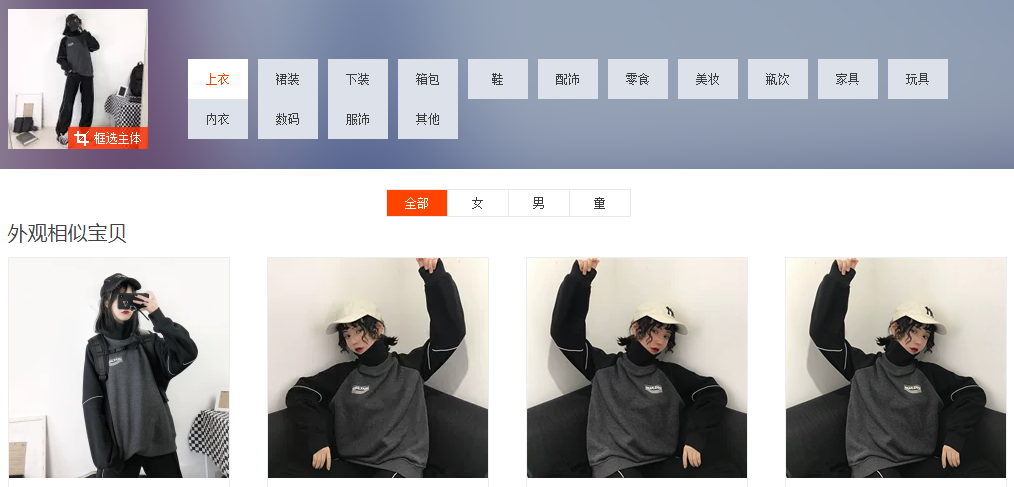
\includegraphics[width = 1\linewidth]{Img/tb.png}
  \caption{淘宝提供的以图搜图功能,用于检索同款商品}
  \label{fig:tb}
\end{figure*}


\section{研究现状}

服装检索的发展经历了两个阶段,分别是基于文本和基于内容的服装检索。基于文
本的服装检索通过关键字或者更加自由形式的文本信息来描述商品,然后通过文本匹
配算法进行服装商品的检索,其本质是以文本搜图。目前,像服装购物平台淘宝等主流
电子商务网站检索服装图像都是以 TBIR(Text-based Image Retrieval)技术为主,TBIR
一般通过关键字检索,其特点是快速精准,但是随着服装种类与数量的不断迅速增长,
TBIR 的不足之处也开始显现出来:现在人们对于服装细节的要求越来越高,然而采用
关键字去标注服装图像无法全面准确的表示服装的细节信息;TBIR 需要人工的对海量
的服装图像做标注,工作量很大;人工标注有时会缺乏客观性,这会直接导致检索结果
的偏差。因此,对基于内容的服装图像检索算法的研究很有必要性,CBIR 通过学习图
像的视觉语义特征进行检索,可以弥补 TBIR 的很多不足。

\subsection{基于视觉特征的服装检索研究现状}

CBIR 算法首先会抽取图像的特征,然后将该特征和检索库里的特征对比,计算相
似度,按照相似性的大小来排序从而可以得到最终的检索结果。初期的 CBIR 算法一般
致力于更好的提取服装的视觉特征,服装是整个服装图像中的主体,因其款式多样、颜
色鲜明、细节突出等特点,相对与自然景象或者生活中其他常见物体等背景信息更加具
有区分度。从服装的这些特点中我们可以抽取服装的纹理、颜色、形状这三大视觉特征,
对这三种特征的提取是初期 CBIR 算法的主要方向:
\begin{itemize}
\item[1.]纹理特征:服装面料最为明显,最具区分性的特征就是纹理,纹理一般情况下以
图像的某种局部特性表现出来,纹理的多样性决定了服装的外在美观程度,更好的提取
服装图片的纹理特征十分有利于检索得到相似度高的服装图像。传统提取纹理特征的方
法主要有四种:频谱法、统计法、结构法和模型法。
纹理特征的提取算法最好具有旋转不变性,Ojala等人提出的LBP纹理分析方法具有旋转不变性的优点,但该方法只使用了服装图像的局部信息去提取特征,没有很好
的利用图像的全局信息\cite{ojala2002multiresolution}
。Manthalkar等人的方法具有旋转不变性和尺度不变性,然而
该方法牺牲了纹理的方向信息\cite{manthalkar2003rotation}。

\item[2.] 颜色特征:颜色是服装的重要构成部分,是图像的一种显著的视觉特征,其对于
图像检索也一直是十分重要的特征。早期对颜色特征的提取主要通过统计图像像素点的
值,近阶段则是偏向于研究图像颜色信息空间分布的检索方法,Pass 等人统计图像中各
颜色最大连续区域的像素值,将其作为颜色特征\cite{pass1996comparing};Strieker 等人将图像划分,再分别
对划分后的各个子区域进行颜色特征的统计提取\cite{stricker1997spectral}。总体的来说,目前基于颜色信息
的检索方法主要考虑对全局以及局部颜色特征的抽取。

\item[3.] 形状特征:形状是决定服装款式多样性的重要因素,蕴含了服装的设计理念和
风格,其对于人的视觉感受也是十分重要的因素。形状特征的提取被广泛应用于 CBIR,
除了如何更好的提取形状特征之外,不同形状特征之间的相似度计算也是近来被探索的
课题。
对形状特征的提取注重关注服装图像的轮廓信息,以及更好的处理区域特征。轮廓
特征指服装的边界形状信息所包含的特征,相关参数有边界点、面积、周长等,相关研
究有 Livarinen 等人提出链码直方图\cite{iivarinen1997comparison};Berretti
等人提出基于平滑曲线分解特征等\cite{berretti2000retrieval}。区域特征指的是图像服装区域内部所包含的信
息,常用矩的方法, Chin等人提出几何不变矩,可以更好地提取形状特征\cite{teh1988image}。对形状特相似性度量的
研究:Peter 等提出 K 最近邻图\cite{kontschieder2009beyond};Bai 等人利用了形状特征之间的相似性与图之间
的相互关系,将形状特征间的相似性构建为图,更有效得去度量形状间相似性\cite{bai2010learning}。

\end{itemize}

\subsection{基于语义特征的服装检索研究现状}
传统的 CBIR 方法采用颜色、形状、纹理等视觉特征,这些特征较为底层,使用的
分类器大多是浅层分类器,如支持向量机。这种基于底层视觉特征的检索系统和人类视
觉体系对图像的理解存在着语义鸿沟,即对于不同的图片,机器从低级的可视化特征得
到的相似性和人从高级的语义特征得到的相似性之间的不同\cite{卢兴敬2008基于内容的服装图像检索技术研究及实现}。所以,即便图像检索
领域在对底层视觉特征的提取有了很大进展,提出了一系列不同的方法,但由于语义鸿
沟的存在,图像检索依然面临着巨大的挑战,我们希望机器可以像人一样理解识别图片
内容,则需要从更高层次去分析图片,现阶段最有希望解决这个语义鸿沟的技术是机器
学习。机器学习是一门涉及统计学、概率论、优化算法等领域的交叉学科,旨在研究如
何让计算机像人一样去学习新的知识,模仿人的行为,不断的通过学习提高自己。机器
学习算法的学习流程是:人为的将大量数据输入到计算机程序,让计算机去处理这些海
量数据,使其发现并总结出这些数据背后所蕴含的规律等隐含信息,机器学习的优势是
可以凭借计算机的高性能计算从大数据中学习得到人类无法轻易总结出的规律。21 世
纪以来,机器学习技术不断发展成熟,应用范围也从开始单纯的字符识别慢慢多样化,
比如生物信息中的基因大数据分析,金融行业中通过对历史数据规律的分析预测市场走
向。

在机器学习中,深度学习技术近年来得到了爆发性的发展,深度学习在计算机视觉、
自然语言处理、多媒体、语音识别等方向均取得了巨大的成功,极大的推动了人工智能
领域的发展进程。深度学习作为机器学习领域的一个分支,起源于 80 年代的 BP \cite{rumelhart1988learning}神经网
络,这是一种对误差逆向传播的多层前馈神经网络,其核心思想是通过梯度下降法不断
优化网络,使得算法不断往误差的最小化方向参数调优。深度学习发展如此迅猛主要得
益于两个方面的原因:计算机的计算能力快速发展,神经网络的训练可以部署在 GPU
上并且可以并行训练,这使得大规模的神经网络可以训练;另一个原因则是大数据的快
速发展,训练数据是机器学习算法的核心之一,随着互联网的发展,日常产生的数据呈
指数级增长,这些海量的标注数据促进了深度学习模型的训练。相对于传统机器学习,
深度学习可以自动的找出分析问题所需要的重要特征,随着神经网络的加深,可以抽取
上层次的语义信息。深度网络中比较有代表性的是卷积神经网络,Lecun 等 提出的
LeNet-5\cite{lecun1998gradient} 在手写字符识别领域的成功应用引起了学术界对于卷积神经网络的关注,2012
年 Alex Krizhevsky 提出 AlexNet\cite{krizhevsky2012imagenet},一举摘下了视觉领域竞赛 ILSVRC 2012 的桂冠,在
百万量级的 ImageNet\cite{deng2009imagenet} 数据集合上,效果大幅度超过传统的方法 [7],这成为卷积神经网
络的一个历史性时刻,AlexNet 之后,不断有新的卷积神经网络模型被提出,从 VGG\cite{simonyan2014very}、
GoogLeNet\cite{szegedy2015going}、Res-Net\cite{he2016deep} 到近期的 Res-NeXt\cite{xie2017aggregated}、SE-Net\cite{hu2018squeeze}。

和基于视觉特征类似,对于区域信息特征的学习是基于语义特征的服装检索一个重
要研究方向,CVPR2016 的工作 Fashion-Net\cite{liu2016deepfashion} 在服装检索中通过关键点信息来对局部特
征进行对齐操作,通过第一步预测出关节点,然后通过关键点信息和池化操作获得对应
的局部特征,这种做法可以较为准确的定位到服装所在区域,但是需要对于关键点的标
注数据进行训练,资源消耗较大。在服装检索的问题上,同款服装的不同图片的相似度
应大于不同款服装的相似度,因此度量学习在网络训练时被广泛使用。常用的度量学习
损失方法有对比损失(Contrastive loss)
、三元组损失(Triplet loss)
、困难样本采样三元
组损失(Triplet hard loss with batch hard mining, TriHard loss)等。除了以度量损失函数
作为网络训练的监督信息以外,服装的低层信息,比如颜色、纹理、形状等也常被作为
辅助监督,这种多任务学习的方式使得网络具有更强的表达能力,学习得到语义信息更
加丰富的特征。

\subsection{研究目标及研究内容}
本课题采用 DeepFashion\cite{liu2016deepfashion} 数据集作为训练集,阿里巴巴 2017 大规模图像搜索大赛
的数据集作为测试集,共 300 万张测试图片。评价标准为上装,裙装和下装的检索 top4
命中率,对应的目标性能分别为 85%、80%、75%。

对于服装图像检索这项任务,局部特征的学习与对齐一直是研究的重要方向,这也
是本课题面临的最大考验。此外,深度学习一直以来都有一个问题:训练好的模型在另
外一个域的性能会下降。针对这两方面的问题,本课题的研究内容如下:
\begin{itemize}
  \item [1.] 基础网络的选择和搭建,随着深度学习发展的快速推进,不同的卷积网络也不断
    的被提出,为了更好学习服装图像特征,借鉴不同网络的设计理念,设计最适合本课题
    数据集的基础网络十分重要。

  \item [2.] 对数据的预处理以及数据扩充,数据集中的图像均来自买家或者卖家拍摄生成,
    这也与实际应用场景一致。但这也会带来一些问题:衣服区域在图像中的位置和比例具
    有很大的不一致性;另外,遮挡、旋转、光照等不确定因素,也会使得图片的质量得不
    到保证。针对这两种情况,首先需要对图像样本做目标检测预处理,针对上述不确定性
    的数据扩充对加强模型的泛化能力也是十分有必要的。

  \item [3.] 更好的结合全局特征和局三部特征,全局特征有着更准确的语义信息,而局部特
    征则是可以提供细粒度的信息,全局特征和局部特征的结合可以大大加强模型的表达能
    力。学好局部特征的关键之一是如何让同款服装的不同图像做到区域间的对齐,采用注
    意力机制使得网络自适应的关注服装的关键细节信息。

  \item [4.] 调研度量学习和多任务学习,在模型训练时引入多个监督以增强模型学习能力。
    利用三元组损失的工作原理,从测试集挖掘样本加入训练集迭代训练,弱化不同域的数
    据测试对模型性能带来的影响。

\end{itemize}
